\chapter{Implementação}
\label{cap5}



Este capítulo visa expressar o funcionamento prático dos microsserviços implementados.
%
Isto é necessário pois as escolhas técnicas, envolvendo as linguagens adotadas, as tecnologias utilizadas e boas práticas aplicadas no desenvolvimento das aplicações, interferem na qualidade dos microsserviços.
%
Denotando-se qualidade como o consumo de recursos e desempenho das aplicações.





Devido as diversas possibilidades de linguagens de programação e bibliotecas disponíveis, a Seção~\ref{sec:tecnologias} tem o objetivo de descrever as tecnologias utilizadas para o desenvolvimento das aplicações e justificar tais escolhas.
%
Além disso, a Seção~\ref{sec:tecnologias} apresenta o conjunto de serviços externos utilizados para facilitar o desenvolvimento dos microsserviços.
%
O serviços externos apesar de não estarem diretamente implementados na arquitetura das soluções, foram utilizados durante o processo e devem ser evidenciados.



Diante da complexidade das arquiteturas de microsserviços desenvolvidos, torna-se necessário descrever quais microsserviços foram implementados, e como estão dispostos na rede.
%
Para este fim, a Seção~\ref{sec:interconexao} contextualiza a interconexão dos microsserviços desenvolvidos.



\section{Tecnologias Utilizadas}
\label{sec:tecnologias}



A seleção das tecnologias e bibliotecas que são executadas nas aplicações é importante, visto que elas implicam diretamente no desempenho e consumo de recursos das arquiteturas selecionadas.
%
Entretanto, essa seleção precisa estar de acordo com as regras de negócio impostas para os testes.



Inicialmente, existe uma preocupação com a linguagem de programação utilizada, visto que ela precisa ter um bom desempenho, um suporte a programação paralela e, ao mesmo tempo, conter bibliotecas que auxiliem no desenvolvimento ágil de tais serviços.
%
Neste sentido, foi levantado um conjunto de linguagens de programação, o qual viabilize o projeto de acordo com os seguintes critérios:



\begin{itemize}
  \item Alto desempenho para programas paralelos;
  \item Biblioteca para conexão com banco de dados PostgreSql;
  \item Biblioteca para uso de cache (Redis);
  \item Biblioteca para escrita de serviços \ac{rpc}, sobre o protocolo \ac{tcp};
  \item Biblioteca para escrita de serviços \textit{web}, com \ac{api} no formato \ac{json};
  \item Linguagem compilada;
  \item Linguagem com tipagem estática; e
  \item Simplicidade de escrita de código, preferencialmente.
\end{itemize}



A partir destes critérios, a linguagem selecionada foi a linguagem GoLang, por se tratar de uma linguagem a qual o autor possui domínio e satisfaz os critérios definidos anteriormente.



Outro critério, o qual é implícito para o desenvolvimento, é a homogenidade da linguagem de programação em todos os microsserviços.
%
Tal necessidade gera o benefício da escrita de código reutilizável, como o núcleo de regras de negócio que pode ser aplicado a todas as arquiteturas desenvolvidas.



Desta forma, foi selecionada uma única linguagem de desempenho compatível com a viabilização do projeto.
%
Em função da diversidade de bibliotecas disponíveis, também é necessário definir quais bibliotecas foram utilizadas para o desenvolvimento das arquiteturas dos microsserviços.
%
Dentre as bibliotecas utilizadas, destacam-se:



\begin{itemize}
  \item gin: Servidor Web para serviços de alto desempenho;
  \item gorm: Biblioteca de objetos relacionais, a qual suporta conexão direta ao banco PostgreSQL;
  \item go-redis: Biblioteca para conexão ao serviço Redis;
  \item net/rpc: Biblioteca nativa da linguagem GoLang para escrita de serviços \ac{rpc} sobre o protocolo \ac{tcp};
  \item graphite: Biblioteca de conexão ao banco de métricas;
  \item testify: Biblioteca auxiliar a suíte nativa de testes da linguagem.
\end{itemize}



Tais bibliotecas foram utilizadas na camada de infraestrutura, sendo seu uso aplicado a todas as arquiteturas.
%
A camada de infraestrutura é responsável pela realização da interação entre a rede e as regras de negócio dos microsserviços.


Destaca-se, dentre as bibliotecas citadas, a biblioteca testify.
%
Tal biblioteca foi utilizada na garantia de integridade das aplicações desenvolvidas.
%
Sua finalidade é realizar a inspeção automatizada do funcionamento da aplicação.
%
Entretanto, a biblioteca não é utilizada durante a execução da aplicação, denotando-se como uma biblioteca auxiliar.



As bibliotecas auxiliares foram utilizadas no processo de integração contínua.
%
O processo de integração contínua foi implantado utilizando os serviços externos Github e TravisCI.
%
Este processo é descrito como processo de construção na arquitetura Willson, sendo responsável pelo teste e envio de imagens de contêineres a um serviço de resgistro na nuvem.




Após descrever as tecnologias utilizadas, faz-se necessário descrever o ambiente distribuído desenvolvido, a fim de garantir uma melhor visibilidade dos microsserviços implementados.



\section{Interconexão entre os microsserviços}
\label{sec:interconexao}



A interconexão entre os microsserviços refere-se ao projeto de rede de uma arquitetura qualquer, disponilizando visualmente a camada de rede.
%
Ao todo foram implementados onze microsserviços, os quais possuem a qual comunicam-se por troca de mensagens.
%
Tais conexões entre sí, com os bancos de dados e com os seus respectivos clientes foram definidas pelos autores das arquiteturas.
%
Consequentemente, torna-se interessante descrever a interconexão entre os microsserviços, exibindo assim seus protocolos de comunicação de rede.



A arquitetura Rudy contém um microsserviço intermediário para conexão com o banco de dados.
%
Esta disposição de microsserviços está exposto na Subseção~\ref{sec:inter_rudy}.



A arquitetura Salz remove a responsabilidade de mensageria do jogo do microsserviço de jogo.
%
Outra alteração é a exposição do microsserviço de autenticação como uma interface pública na rede, permitindo a conexão a partir dos clientes.
%
Esta disposição de microsserviços da arquitetura Salz é descrito na Subseção~\ref{sec:inter_salz}.



A arquitetura Willson tem o funcionamento semelhante a arquitetura Rudy, porém não utiliza um microsserviço intermediário para organização de consultas ao banco de dados.
%
A disposição dos microsserviços nesta arquitetura é visível na Subseção~\ref{sec:inter_willson}.



\subsection{Rudy}
\label{sec:inter_rudy}


A arquitetura Rudy em versão reduzida para o escopo dos testes contém quatro microsserviços e dois banco de dados, sendo um para dados permanentes (PostgreSQL) e um para cache (Redis).
%
Os seus microsserviços estão listados na Tabela~\ref{tab:inter_rudy}.

\begin{table}[htb!]
\centering
\begin{adjustbox}{max width=\textwidth}
\caption{Microsserviços da arquitetura Rudy.}
\label{tab:inter_rudy}
\begin{tabular}{l|l|l}
\hline
Nome            & Protocolo            & Público a Rede \\ \hline
 rgame          & \ac{rpc}/\ac{tcp}    & \checkmark     \\ \hline
 rweb           & \ac{http}/\ac{json}  & \checkmark     \\ \hline
 rauth          & \ac{rpc}/\ac{tcp}    &                \\ \hline
 rcrud          & \ac{rpc}/\ac{tcp}    &                \\ \hline
\end{tabular}
\end{adjustbox}

Fonte: O próprio autor.
\end{table}


A arquitetura Rudy contém um microsserviço especial intermediário para conexão com o banco de dados.
%
O seu principal objetivo é concentrar todas as chamadas para o banco de dados, minimizando erros ao acessar os dados.
%
Esta característica especial é visível na Figura~\ref{fig:interconexao_rudy}.



\begin{figure}[htb!]
  \caption{Interconexões da arquitetura Rudy.}
  \label{fig:interconexao_rudy}
  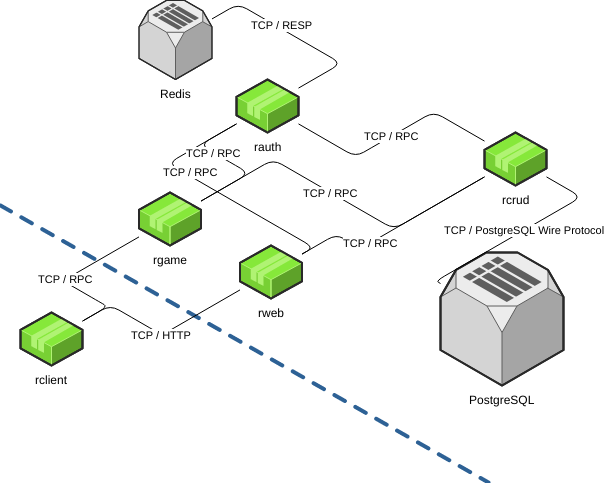
\includegraphics[width=0.8\textwidth]{figuras/interconexoes/rudy.png}
  \centering

  Fonte: O próprio autor.
\end{figure}



Conforme exibido na Figura~\ref{fig:interconexao_rudy}, existe uma camada sobressalente interceptando o acesso ao banco.
%
Esta camada tende a aumentar o tempo de resposta de requisições ao acessar os dados, no entanto, permite também o controle refinado de acesso.


\subsection{Salz}
\label{sec:inter_salz}


Na arquitetura Salz, as conexões com o banco de dados são feitas sem interceptores, ou seja, sem a utilização de um microsserviço intermediário.
%
Além disso, esta arquitetura divide o microsserviço de jogo entre os microsserviços de Chat e Jogo.
%
Esta abstração tende a reduzir o consumo de recursos de uma instância, permitindo mais conexões simultâneas sem estressar o serviço de jogo.
%
A arquitetura Salz pode ser observada na Figura~\ref{fig:interconexao_salz}.



\begin{figure}[htb!]
  \caption{Interconexões da arquitetura Salz.}
  \label{fig:interconexao_salz}
  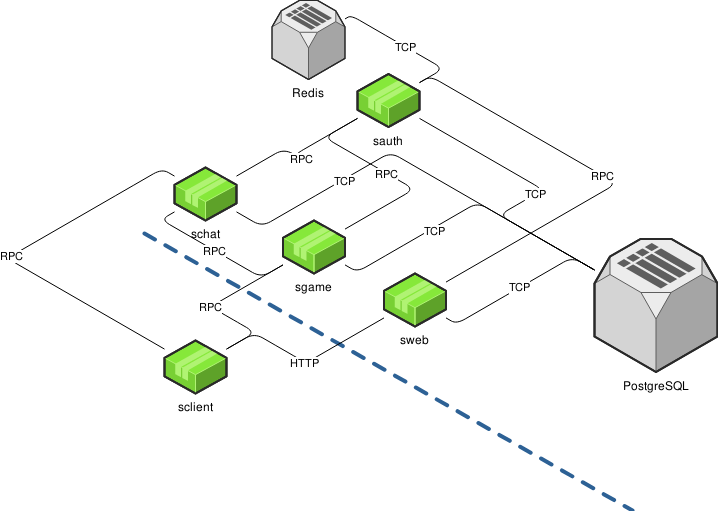
\includegraphics[width=0.8\textwidth]{figuras/interconexoes/salz.png}
  \centering

  Fonte: O próprio autor.
\end{figure}



A interconexão da arquitetura Salz, exibida na Figura~\ref{fig:interconexao_salz}, contém três conexões simultâneas.
%
As triplicidade de conexões evita a necessidade de sincronização dos estados de jogo entre os microsserviços.
%
Entretanto, alguns dados ainda precisam ser consultados, como a posição dos personagens no mundo, para verificação de distância ao envio do chat.
%
Por este motivo, espera-se que a transmissão de dados destes serviços seja mais intensa em relação a outros serviços.


A compensação deste aumento de transmissão de dados elevado entre o chat e o serviço de jogo pode ser executada pela falta de um serviço intermediário ao banco.
%
Diante desses fatos, torna-se interessante a análise desta característica, visto que tal característica pode ter um impacto positivo para o consumo dos recursos da arquitetura.


\subsection{Willson}
\label{sec:inter_willson}


A arquitetura Willson é destacada pela eliminação de microsserviços intermediários.
%
Essa abordagem evita a troca de mensagens entre serviços intermediários, tendo seu objetivo a diminuição do tempo de resposta.
%
A arquitetura Willson pode ser observada na Figura~\ref{fig:interconexao_willson}.



\begin{figure}[htb!]
  \caption{Interconexões da arquitetura Willson.}
  \label{fig:interconexao_willson}
  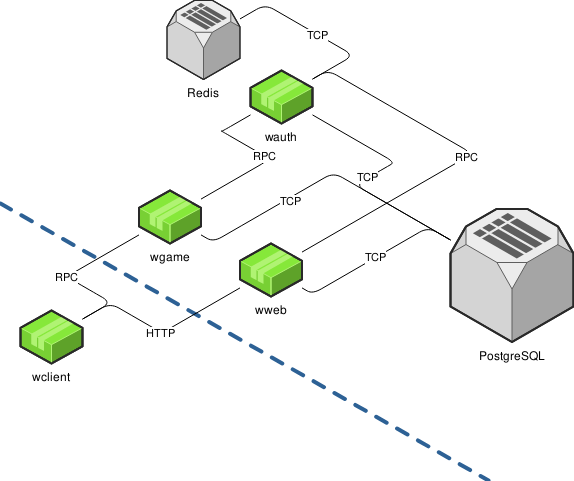
\includegraphics[width=0.8\textwidth]{figuras/interconexoes/willson.png}
  \centering

  Fonte: O próprio autor.
\end{figure}



A interconexão da arquitetura Willson, exibida na Figura~\ref{fig:interconexao_willson}, é projetada para reduzir o número de trocas de mensagens.
%
Desta forma, espera-se ter um consumo da rede inferior em relação as demais arquiteturas. Este ponto também deve ser analisado.
